% Template for a Thesis
%
% 4-translation.tex
%
% Translation

\chapter{Translation}\label{ch:translation}

A significant component of this thesis is the use of word alignments, a method eployed in satistical machine translation in order to gauge how good a translation is. If a word in French gets aligned to its equivalent word in English, for example \emph{maison-house}, then the translation is correct. It is a metric to evaluate if a translation has been successful.

This thesis is not related to translation, not SMT nor its more modern approach neural machine translation. But the word alignment algorithm is used in order to compare word alignments against BPE alignments. Taking word alignments as the basis, alignment algorithms are used to see if these BPE units are also correctly aligned to the BPE units in the other language. For example, ideally the English suffix \emph{ment} would be aligned to the German word ending of \emph{keit}. But before diving deep into word alignments and how they work, it is important to understand the background of this algorithm, as well as its original purpose and a general notion of how statistical machine translation works.

\section{Statistical machine translation (SMT)}

SMT is a machine translation approach where translations are generated based on statistical models, whose parameters are derived from the analysis of bilingual text corpora. It can be done with rule-based approaches in a supervised way, or example-based approaches, in an unsupervised way. A document is translated according to the probabilistic distribution \emph{P(e|s)} that a word \emph{e} in the target language (for example English) is the translation of a word \emph{s} in the source language (for example, Spanish).

\begin{itemize}
	\item Suppose that s = gracias
	\item P(thanks|gracias) = 0.45
	\item P(appreciate|gracias) = 0.13
	\item P(water|gracias) = 0.00001
\end{itemize}

Given the word \emph{gracias}, the translation algorithm would give a higher probability that it is aligned with \emph{thanks}, and lower probabilities to other alignments. For each word, there usually is a list with alignment possibilities and its probabilities, and the one with the highest probability is taken as alignment. Note that since this translation method is statistical, there is no direct translation, there is no direct approval of one alignment and dismissal of the rest, since all is based on probabilities.

Typically, a translation model first translates the source language into a broken version of the target language, using an algorithm such as the expectation-maximization algorithm. Afterwards, a language model in the target language makes the broken language look more natural, in the way native speakers would speak it. A good language model will for example assign a higher probability to the sentence "the house is small" than to "small the is house". An example of a translation system from Spanish to English can be seen in Figure  4.1. In the first step, the translation model needs to know which words to align in a source-target sentence pair, which is handled by the word alignment step.

\begin{figure}[!ht]
    \centering
    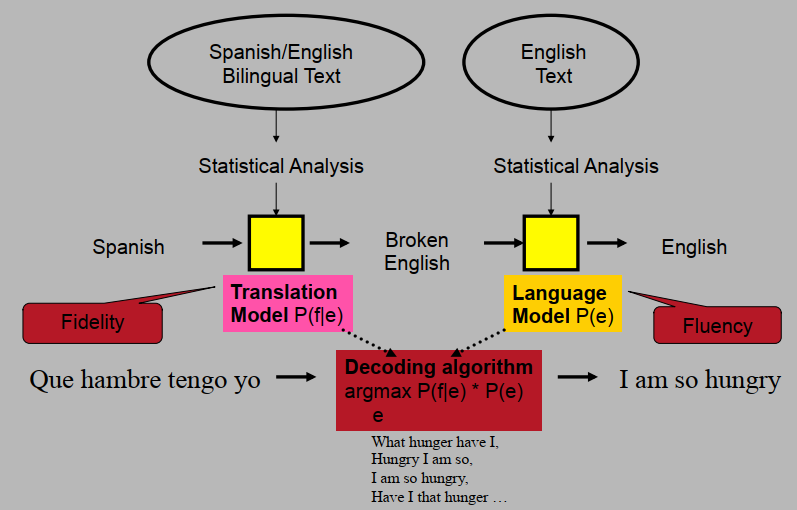
\includegraphics[width=11cm]{figures/smt.png}
    \caption{Example of Spanish-English SMT system.}
\end{figure}

\section{Word alignments}

Word alignment between a parallel corpora is the NLP task of identifying translation relationships among the words in a parallel text, resulting in a graph between the two sides of the texts, with an arc between two words if they are translations of one another. Figure 4.2. shows an alignment example between a sentence in English and its counterpart in French. Alternatively, the alignments can also be displayed in a matrix as shown in Figure 4.3.

\begin{figure}[!ht]
    \centering
    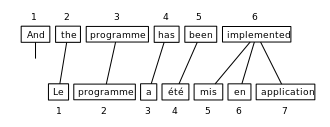
\includegraphics[width=10cm]{figures/word_align.png}
    \caption{Word alignments between an English and French sentence.}
\end{figure}

\begin{figure}[!ht]
    \centering
    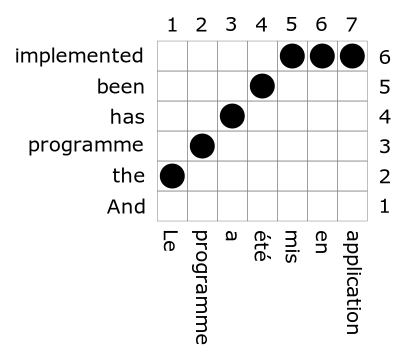
\includegraphics[width=6cm]{figures/word_align_matrix.png}
    \caption{Word alignments between an English and French sentence in matrix form.}
\end{figure}

The most basic words usually have one-to-one alignments, such as \emph{the-le} in this example, and words with the same root, \emph{programme-programme} since they both come from Latin. However, in many cases one language might express something using one word but another might express with with many words, distributed throughout the sentence. Besides, as seen in this example, some words do not even have an alignment (\emph{And}), and some have multiple alignments, in this case one-to-many: \emph{inmplemented-mis en application}. There can also be many-to-one and many-to-many alignments.

The parameters of word alignment methods are usually estimated by observing word-aligned texts~\cite{brown1993mathematics}, and automatic word alignment is typically done by choosing that alignment which best fits a statistical machine translation model. A popular algorithm to find word alignments is the \textbf{expectation-maximization algorithm}~\cite{och1999improved}

For training, historically IBM models have been used.~\cite{koehn2009statistical} These models are used in statistical machine translation to train a translation model, as well as an alignment model. They make use of the expectation-maximization algorithm explained above: in the expectation step, the translation probabilities within each sentence are computed; in the maximization step, these probabilities are accumulated to global translation probabilities.

This approach is an example of unsupervised learning, meaning that the system has no knowledge of the kind of output it is expected to produce, but tries to find values for the unobserved model and alignments which best explain the observed parallel text. In some cases, a small number of manually aligned sentences is used to help the model, as a way to explore supervised learning.~\cite{varga2007parallel} These models are able to more easily take advantage of combining many features within the data, such as context, syntactic structure, part-of-speech or translation lexicon information, which are difficult to integrate into the unsupervised models generally used.

\subsection{Fastalign algorithm}

Fastalign algorithm~\cite{dyer-etal-2013-simple} is a simple log-linear reparametrization of IBM Model 2 that overcomes problems from both Model 1 and Model 2. Training this model is consistently ten times faster than Model 4. An open-source implementation of the alignment model described in this paper is available in \href{http://github.com/clab/fast align}{Github}.

Fastalign is a variation of the lexical translation. Lexican translation works as follows: given a source sentence \emph{f} with length \emph{n}, first generate the length of the target sentence \emph{m}, where the target sentence is \emph{e}. Then generate an alignment vector of length \emph{m} that indicates which source word (or null token) each target word will be a translation of. Lastly, generate the \emph{m} output words, where each word in \emph{e} depends only on the word in \emph{f} it's aligned with.

Fastalign's modification is that the distribution over alignments is parametrized by a null alignment probability and a precision parameter, which controls how strongly the model favors alignment points close to the diagonal (if we use the word alignment matrix like in the example above). It also adds a symmetrization step called GDFA.

The paper~\cite{dyer-etal-2013-simple} has more detailed information on training, inference and results.

\subsection{Eflomal algorithm}

The Eflomal alignment algorithm~\cite{ostling2016efficient}, presented in 2016, defins itself as an \emph{Efficient Low-Memory Aligner}. Its code is available \href{https://github.com/robertostling/eflomal}{on Github}, and it is a word alignment tool based on efmaral, with some improvements, such as more compact data structures, yielding a lower memory requirement, and the fact that the estimation of alignment variable marginals is done one sentence at a time, which also saves a lot of memory at no detectable cost in accuracy. Eflomal differs from Fastalign in the sense that it is based on a hidden Markov Model, as opposite to Fastalign which is based on an IBM model. Eflomal also requires the simmetrization step GDFA, and has historically had better results than Fastalign. Technical details relevant to both efmaral and eflomal can be found in the cited article.

\section{Alignment metrics}\label{tra:metrics}

Evaluating alignments is usually done by the following metrics: precision, recall, F1 score and accuracy. It is assumed that the actual results are at a disposal, in this case, that the correct alignments are known. The system then makes a prediction for certain alignments. This confusion matrix shows th etable for true positives, true negatives, false positives and false negatives.

\begin{figure}[!ht]
    \centering
    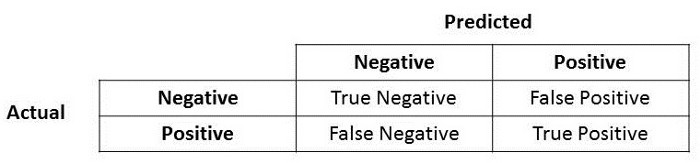
\includegraphics[width=12cm]{figures/precrec.jpeg}
    \caption{Confusion matrix for actual and predicted results}
\end{figure}

If an alignment is predicted and is also correct, that constitutes a true positive. If an alignment is predicted but is not correct, that constitutes a false positive. If a correct alignment was not predicted, it constitutes a false negative. And an alignment that is not present in the actual alignment list nor in the prediction list is a true negative. These are the formulas to calculate the precision, recall and F1 score:

\begin{itemize}
    \item Precision =  true positives / (true positives + false positives) = true positives / (total predicted positives)
    \item Recall =  true positives / (true positives + false negatives) = true positives / (total actual positives)
    \item F1 score = 2 x precision x recall / (precision + recall)
\end{itemize}

In a nutshell, precision evaluates the following: out of all the predicted items, how many are correct? And recall: out of all the correct items, how many were predicted? The F1 score is a balance between the two, so that a system with a high precision but low recall might have a decent F1 score.

This is the traditional use of precision and recall. When talking specifically about alignments however, a slightly different definition is commonly provided:

\begin{itemize}
    \item Precision =  test alignments x possible alignments / test alignments
    \item Recall =  test alignments x sure alignments / sure alignments
    \item F1 score = (test x sure + test x possible) / (test + sure)
    \item AER = 1 - F1 score
\end{itemize}

AER, Alignment Error Rate~\cite{mihalcea2003evaluation}~\cite{koehn2009statistical}, is a commonly used metric for assessing sentence alignments. It combines precision and recall metrics together such that a perfect alignment must have all of the sure alignments and may have some possible alignments. It is the opposite of the F1 score.

